\documentclass[12pt]{article}
 
\usepackage[margin=1in]{geometry} 
\usepackage{amsmath,amsthm,amssymb}
\usepackage{hyperref}
\usepackage{graphicx}
\usepackage{xcolor}
\usepackage[many]{tcolorbox}
\tcbuselibrary{listings}
\usepackage{listings}
\usepackage{float}

\definecolor{lg}{HTML}{f0f0f0}

\newtcblisting{pycode}{
    colback=lg,
    boxrule=0pt,
    arc=0pt,
    outer arc=0pt,
    top=0pt,
    bottom=0pt,
    colframe=white,
    listing only,
    left=15.5pt,
    enhanced,
    listing options={
        basicstyle=\small\ttfamily,
        keywordstyle=\color{blue},
        language=Python,
        showstringspaces=false,
        tabsize=2,
        numbers=left,
        breaklines=true
    },
    overlay={
        \fill[gray!30]
        ([xshift=-3pt]frame.south west)
        rectangle
        ([xshift=11.5pt]frame.north west);
    }
}

\lstset{
    language=Python,
    basicstyle=\small\ttfamily,
}

 
\begin{document}
 
\title{Exercise 6}
\author{Cristian Manuel Abrante Dorta - 888248\\
ELEC-E8125 - Reinforcement Learning}

\maketitle
\section{Actor critic with episodic updates}

\subsection{Task 1:}
\textbf{
Revisit the policy gradient solution for the continuous Cartpole from Exercise 5 with learned sigma and implement the actor-critic algorithm.
}\\

In Figure \ref{fig:task-1} we can see the performance of the training of the Actor-Critic algorithm.

\begin{figure}[ht]
    \centering
    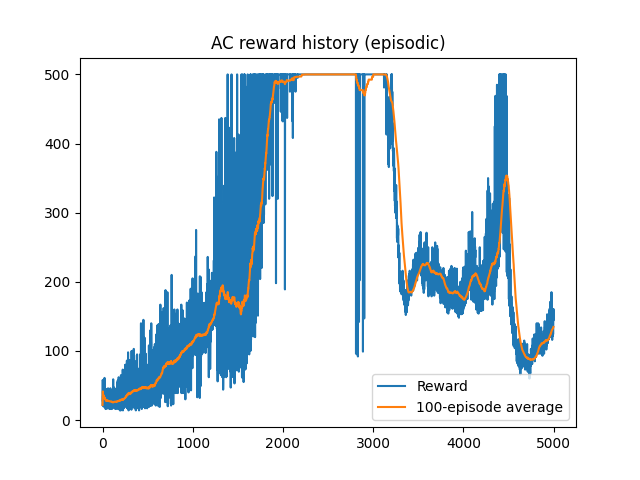
\includegraphics[scale=0.5]{exercise-6/plots/exefcise-6-good-1.png}
    \caption{Training plot for Actor-Critic with episodic updated}
    \label{fig:task-1}
\end{figure}

In the plot it can be observed that the agent is able to drastically improve the rewards obtained, and this is really significant from episode 2000, when the maximum of 500 timesteps is achieved. After that, the performance of the agent is reduced, having a incremental peek at the end of the 2000 episodes.

\subsection{Question 1}
\textbf{What is the relationship between actor-critic and REINFORCE with baseline?}

For explaining the relation between the two methods, first we are going to explain the different objective functions. In the case of the simple REINFORCE method, the objective function is calculated with this expression:

\begin{equation}
    \nabla_\theta J(\theta) = \sum^{T-1}_{t=0}\nabla_\theta log\pi_\theta(a_t|s_t)G_t
\end{equation}

Where the term $G_t$ is the expected rewards obtained in time $t$. This term has a high variance because the different trajectories that the agent follows during the training can diverge between each other in a significant way. Baseline term is introduced then for reducing the amount of variance of the expected reward term. SO the new objective function is:

\begin{equation}
    \nabla_\theta J(\theta) = \sum^{T-1}_{t=0}\nabla_\theta log\pi_\theta(a_t|s_t)(G_t - b(s_t))
\end{equation}

Actor-critic methods are based on the same idea, but they use a more sophisticated method, which can also combine the action value. This idea is that we can use the q-value of the state and action as an approximation of the term $G_t$, converting the previous expression in:

\begin{equation}
    \nabla_\theta J(\theta) = \sum^{T-1}_{t=0}\nabla_\theta log\pi_\theta(a_t|s_t)Q(s_t, a_t)
\end{equation}

So the new objective function for actor-critic could be estimated using two neural networks, the first network is used for estimate the policy (as in the REINFORCE algorithm), being the \textit{actor} part, and the second network is used for estimate the Q-value function, being the \textit{critic} part. \\

It is important also to say that in practice the Q-value function is not estimated, but instead it is estimated the action-value function because it is more convenient when used with continuous spaces. This applies a TD update for the weights of the network:

\begin{equation}
    A(s_t, a_t) = Q(s_t, a_t) - V(s_t) = r_{t+1} + \gamma V(s_{t+1}) - V(s_t)
\end{equation}

\subsection{Question 2}
\textbf{How can the value of advantage be intuitively interpreted?} \\

The most direct interpretation is that the value of the advantage is the subtraction of the value of taking an action in a certain state minus the expected value of this state. But other interpretation can be extracted using this equation

\begin{equation}
    A(s_t, a_t) = r_{t+1} + \gamma V(s_{t+1}) - V(s_t)
\end{equation}

This equation uses only the action-value of the state, and we can say that what we subtract here is the \textit{more real} version of the action value (in the left part of the minus), because it is the actual reward obtained plus the discounted version of the value of the next state, minus the \textit{estimated} action value of the state (in the right part of the minus).

\section{Actor critic with non-episodic updated}

\subsection{Task 2}
\textbf{Update the actor-critic code to perform TD(0) updates every 50 timesteps, instead of updating your network at the end of each episode. }

After updating the actor-critic to perform the updated every 50 timesteps the following plot was obtained:

\begin{figure}[ht]
    \centering
    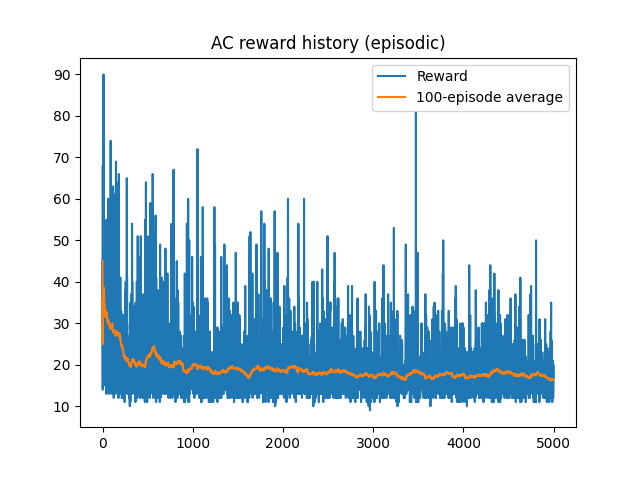
\includegraphics[scale=0.5]{exercise-6/plots/task-2.png}
    \caption{Caption}
    \label{fig:task-2}
\end{figure}

In the following plot, we see that the agent is not able to learn the policy, mainly because the update is done each 50 timesteps, so the episode maybe was not finished and all the histories of the learning is already clean when the network is going to be updated.

\section{Actor critic with parallel data collection}

\subsection{Task 3}
\textbf{Update your code to use parallel data collection.}\\

After training the \texttt{parallel\_cartpole.py} script, the following plot was obtained:

\begin{figure}[ht]
    \centering
    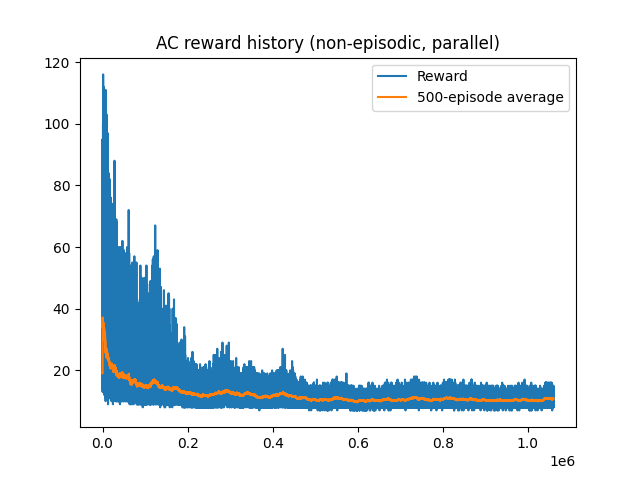
\includegraphics[scale=0.5]{exercise-6/plots/task-3.png}
    \caption{Plot obtained with execution of parallel data collection}
    \label{fig:task-3}
\end{figure}

\subsection{Question 3}
\textbf{How is parallel data collection different from the parallelism in multiple\_cartpoles.py script we’ve seen in Exercises 1 and 5? Can it replace multiple runs of the training algorithm for comparing RL algorithms?}\\

Parallel data collection is different from the parallelism that the script \texttt{multiple\_carpole.py} used. In the latter script, what it is done is to run multiple independent instances of the algorithm, but on the other hand, in parallel data collection, data is obtained from the different cores of the CPU independently, and all this data is used by the same instance of the algorithm.\\

Parallel data collection try to increase the variety of the data used to train the agent but can not substitute the effect of having multiple runs of the algorithm, because with only one run, the neural networks of the agents are trained in a certain way, even though are imporved with data that comes from different sources. On the contrary, with the other approach, neural networks are trained several times, so it is a better reflection of the actual performance of the system.

\subsection{Question 4}
\textbf{Figure 1 shows the training performance for all three actor-critic variants and the REINFORCE algorithm from the last lecture. In terms of initial performance, REINFORCE seems to completely outperform all tested A2C flavours on Cartpole, despite being a simpler algorithm. Why is it so? }\\

This is because the the complexity of the actor-critic algorithm requires more timesteps for the agent to learn how to optimize the rewards. This is because in actor critic are needed two neural networks (the \textit{actor} network and the \textit{critic} network), and both of the networks are dependent between each other. This is a complex pattern that takes more episodes to be learnt.\\

This is also the reason why for training this actor-critic system are needed more episodes compared to the policy gradient (REINFORCE) algorithm.

\subsection{Question 5.1}
\textbf{How do actor-critic methods compare to REINFORCE in terms of bias and variance of the policy gradient estimation? Explain your answer.}\\

In term of variance, actor-critic methods are better than the simple simple REINFORCE algorithm without baseline. This is because, as it was explained in Question 1, when using the expected rewards term directly ($G_t$) for the computation of the objective optimization function, we carry a lot of variance due to the divergence between the possible trajectories that are followed by the agent during the training. On the contrary, when applied actor-critic methods, the divergence between the trajectories is reduced because we compute advantage terms instead of the raw expected rewards. Additionally, as it was defined in question 2, the advantage term is a subtraction between two similar terms (the idea is to have lower difference between both terms). \\

When speaking about the bias of the model, we can say that both REINFORCE and Actor critic are unbiased. This is because if the original REINFORCE model was unbiased, then the introduction of the baseline (which is the basis of actor-critic methods) does also not introduce bias in the model, because the multiplication of the gradient of $\log \pi_\theta(a_t|s_t)$ multiplied by the baseline term $b$ is zero. \\

This is the original expectation with the baseline:

\begin{equation}
    \nabla_\theta \mathbb{E}_{\tau \sim \pi_\theta}[J(\theta)] =
\mathbb{E}_{\tau \sim \pi_\theta} \left[ \sum_{t=0}^{T-1} \nabla_\theta \log
\pi_\theta(a_t|s_t) \left(G_t - b(s_t)\right) \right]
\end{equation}

Which can be expressed as:

\begin{equation}
    \nabla_\theta \mathbb{E}_{\tau \sim \pi_\theta}[R(\tau)] =
\mathbb{E}_{\tau \sim \pi_\theta} \left[ \sum_{t=0}^{T-1} \nabla_\theta \log
\pi_\theta(a_t|s_t) \left(\sum_{t'=t}^{T-1}r_{t'}\right) - \sum_{t=0}^{T-1}
\nabla_\theta \log \pi_\theta(a_t|s_t) b(s_t) \right]
\end{equation}

For proving that the baseline does not introduce bias, what we have to prove is that $\nabla_\theta \log \pi_\theta(a_t|s_t) b(s_t) = 0$, and that can be shown as:

\begin{align}
\mathbb{E}_{\tau \sim \pi_\theta}\Big[\nabla_\theta \log \pi_\theta(a_t|s_t) b(s_t)\Big] &=  \mathbb{E}_{s_{0:t},a_{0:t-1}}\Big[ \mathbb{E}_{s_{t+1:T},a_{t:T-1}} [\nabla_\theta \log \pi_\theta(a_t|s_t) b(s_t)]\Big] \\
&= \mathbb{E}_{s_{0:t},a_{0:t-1}}\Big[ b(s_t) \cdot \underbrace{\mathbb{E}_{s_{t+1:T},a_{t:T-1}} [\nabla_\theta \log \pi_\theta(a_t|s_t)]}_{E}\Big] \\
&= \mathbb{E}_{s_{0:t},a_{0:t-1}}\Big[ b(s_t) \cdot \mathbb{E}_{a_t} [\nabla_\theta \log \pi_\theta(a_t|s_t)]\Big] \\
&= \mathbb{E}_{s_{0:t},a_{0:t-1}}\Big[ b(s_t) \cdot 0 \Big] = 0
\end{align}

\subsection{Question 5.2}
\textbf{How could the bias-variance tradeoff in actor-critic be controlled?}\\

For the reduction of the variance in the actor-critic method, we calculate the advantage terms, thus only the action-value is calculated from the neural network. And this is compared with the sum of the instant reward and the action-value of the future state. Apart from that, it is importance to take into consideration the variance of the generation of random action, controlled by the parameter $\sigma$, of the random distribution generated by the policy network. For this case, the approach followed was adding this parameter to the neural network.

\subsection{Question 6}
\textbf{What are the advantages of policy gradient and actor-critic methods compared to action-value methods such as Q-learning? Explain your answer.}\\

We have two main families of reinforcement learning algorithms. On the one hand, we have value based algorithms, which tries to estimate the value for each state, where the most famous one is Q-Learning and all its variances, the main advantage of them is their sample-efficiency and their steadity. On the other hand, we have the policy gradient methods, such as REINFORCE algorithm, which are based on the calculation of the optimal policy, and their main advantage is their convergence time, and that they are really good for being used with stochastic environments.\\

Actor-critic methods try to merge both methods, using two neural networks, for estimating the policy and the action value. Each of the network is going to learn from the feedback of the other. The result is that the overall system will learn how to optimize the rewards, without requiring so much data as temporal difference methods, and also with the possibility of handling countinous and stochastic action spaces, on the contrary of action-value methods.

\end{document}
